% paper/sections/casestudies.tex — Case Studies section shell
% Written in Phase 89 (Plan 01); revised in the referee pass (generated numbers).
% Each per-study subsection is owned by its own \input file.
% Wave-2 studies (2--4) each add their own casestudyN.tex; this file is FINAL.
\section{Case Studies}
\label{sec:casestudies}

The four studies below illustrate \texttt{fdars} on real datasets spanning
smoothing and functional principal component analysis, elastic registration
with scalar-on-function regression, functional time-series forecasting, and
composable scikit-learn pipelines with hyperparameter search.  Each study is
reproduced by a committed \texttt{paper/code/casestudyN.py} script that
generates the accompanying figures and writes every number quoted in the text
to a \LaTeX{} macro file (\texttt{paper/sections/csN\_numbers.tex}); a CI drift gate
recomputes the numbers and fails if a committed macro file is stale.  Figure
generation is deterministic: re-running a script in the same environment
reproduces its figures byte for byte.

% paper/sections/casestudy1.tex — Case Study 1: Phoneme (smoothing, FPCA, classification)
% Every number below is a macro written by paper/code/casestudy1.py into
% sections/cs1_numbers.tex (drift gate: paper/code/check_cs_numbers.py).
% Auto-generated by paper/code/casestudy1.py -- do not edit.
% Regenerate: PYTHONPATH=scripts:paper/code python paper/code/casestudy1.py
% Drift gate: PYTHONPATH=scripts:paper/code python paper/code/check_cs_numbers.py
\newcommand{\csOneNCurves}{400}
\newcommand{\csOneNPerClass}{80}
\newcommand{\csOneNClasses}{5}
\newcommand{\csOneNFull}{4{,}509}
\newcommand{\csOneNPoints}{256}
\newcommand{\csOneSmoothNBasis}{15}
\newcommand{\csOneSmoothN}{20}
\newcommand{\csOneRawShown}{3}
\newcommand{\csOneNComp}{4}
\newcommand{\csOneVarPCOne}{55.6}
\newcommand{\csOneVarPCTwo}{18.4}
\newcommand{\csOneVarPCThree}{4.4}
\newcommand{\csOneVarPCFour}{1.9}
\newcommand{\csOneCumVarThree}{78.4}
\newcommand{\csOneCumVarFour}{80.3}
\newcommand{\csOneCVAcc}{88.3}
\newcommand{\csOneCVFolds}{0.900, 0.875, 0.813, 0.938, 0.888}
\newcommand{\csOneCVAccFPCLDA}{88.3}
\newcommand{\csOneRecallAa}{58}
\newcommand{\csOneRecallAo}{53}
\newcommand{\csOneRecallDcl}{77}
\newcommand{\csOneRecallIy}{67}
\newcommand{\csOneRecallSh}{79}
\newcommand{\csOneAaAoConfused}{42}
\newcommand{\csOneAaAoTotal}{160}


\subsection{Smoothing, FPCA, and Classification: Phoneme Data}
\label{subsec:cs1-phoneme}

We use a balanced, seeded subset of the phoneme log-periodogram data of
\citet{hastie_buja_tibshirani_1995}: \csOneNCurves{} of the \csOneNFull{} curves
in the file distributed with \emph{The Elements of Statistical Learning},
\csOneNPerClass{} from each of \csOneNClasses{} phoneme classes (\textit{aa},
\textit{ao}, \textit{dcl}, \textit{iy}, \textit{sh}; drawn with \texttt{numpy}
seed~0), each recorded at \csOneNPoints{} frequency points.  (A related version
of these data is analysed by \citet{ferraty_vieu_2006}.)  Results on this
subset are therefore not directly comparable with published results on the
full data.  Each curve is a digitised acoustic spectrum, and the
classification task is to recover the phoneme class from its spectral shape.
This study demonstrates three core \texttt{fdars} capabilities in sequence:
penalised smoothing, functional principal component analysis (FPCA), and
cross-validated classification.

\paragraph{Smoothing.}
Raw log-periodogram curves carry measurement noise.  We apply roughness-penalised
B-spline smoothing (\texttt{fdars.basis.smooth\_basis\_gcv}) with
\csOneSmoothNBasis{} basis functions to a representative subset of
\csOneSmoothN{} curves, selecting the penalty automatically via generalised
cross-validation \citep{craven_wahba_1979,ramsay_silverman_2005}.
Figure~\ref{fig:cs1-smooth} shows the raw spectra alongside the fitted smooth
curves for each class; the smoothed curves retain the phoneme-specific spectral
peaks while suppressing high-frequency noise.

\paragraph{FPCA.}
FPCA is performed on all \csOneNCurves{} curves via
\texttt{Fdata.to\_pc(n\_comp=\csOneNComp)} \citep{ramsay_silverman_2005}.  The
first four principal components explain
$[\csOneVarPCOne, \csOneVarPCTwo, \csOneVarPCThree, \csOneVarPCFour]\%$ of
the total (quadrature-weighted) variance: \csOneCumVarThree\% jointly for the
first three and \csOneCumVarFour\% for all four.  The scores scatter in
Figure~\ref{fig:cs1-fpca} shows that \textit{dcl}, \textit{sh} and, largely,
\textit{iy} separate clearly in the PC1--PC2 plane, whereas the acoustically
similar vowels \textit{aa} and \textit{ao} overlap substantially: a
cross-validated linear discriminant on the first two scores alone recovers
\csOneRecallDcl{}, \csOneRecallSh{} and \csOneRecallIy{} of the
\csOneNPerClass{} \textit{dcl}, \textit{sh} and \textit{iy} curves, but
confuses \textit{aa} and \textit{ao} with each other in \csOneAaAoConfused{}
of their \csOneAaAoTotal{} curves.

\paragraph{Classification.}
We evaluate a scikit-learn \texttt{Pipeline} that chains an \texttt{fdars}
\texttt{FPCATransformer} (\csOneNComp{} components) with scikit-learn's
\texttt{LinearDiscriminantAnalysis} by 5-fold stratified cross-validation, so
that FPCA is fitted once per training fold.  The pipeline achieves a mean CV
accuracy of \csOneCVAcc\% on held-out data (fold scores:
$[\csOneCVFolds]$); the one-step \texttt{fdars} classifier
\texttt{FPCLDAClassifier(ncomp=\csOneNComp)}, which performs the FPCA
internally, gives the same mean accuracy (\csOneCVAccFPCLDA\%) on the same
folds.  The remaining errors are concentrated in the \textit{aa}/\textit{ao}
pair noted above.
The analysis, including every number above, is reproduced by
\texttt{paper/code/casestudy1.py}, which also generates both figures
deterministically.

\begin{figure}[tbp]
  \centering
  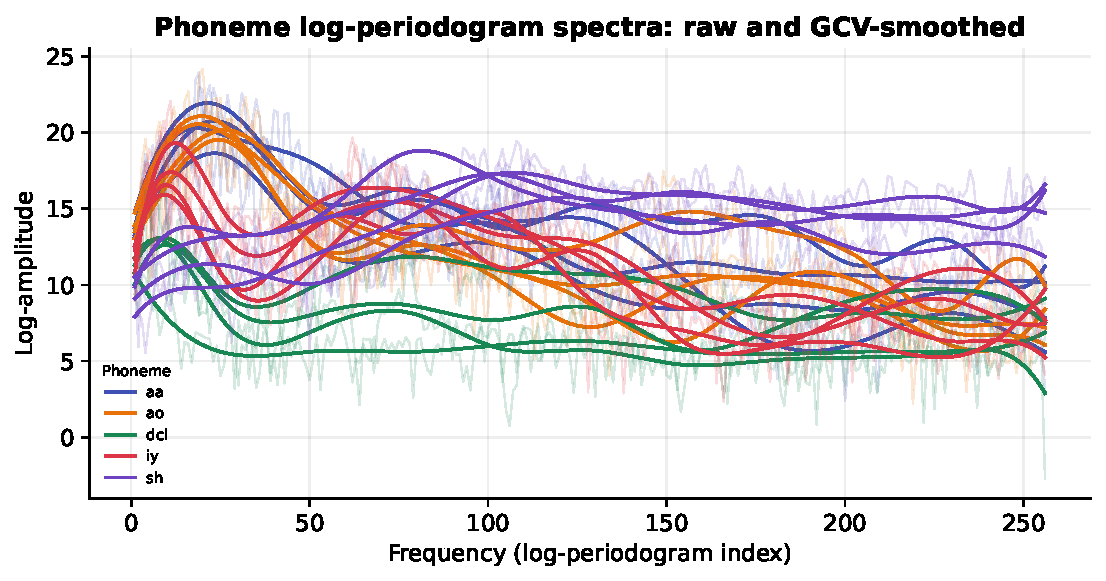
\includegraphics[width=\textwidth]{figures/cs1_phoneme_smooth.pdf}
  \caption{Phoneme log-periodogram spectra (balanced \csOneNCurves-curve subset,
    \csOneNClasses{} classes).  Light traces: raw curves (\csOneRawShown{} per
    class); bold traces: GCV B-spline smoothed curves (\csOneSmoothNBasis{}
    basis functions, penalty selected by GCV\@).  Colours identify phoneme
    classes (\textit{aa}, \textit{ao}, \textit{dcl}, \textit{iy},
    \textit{sh}).}
  \label{fig:cs1-smooth}
\end{figure}

\begin{figure}[tbp]
  \centering
  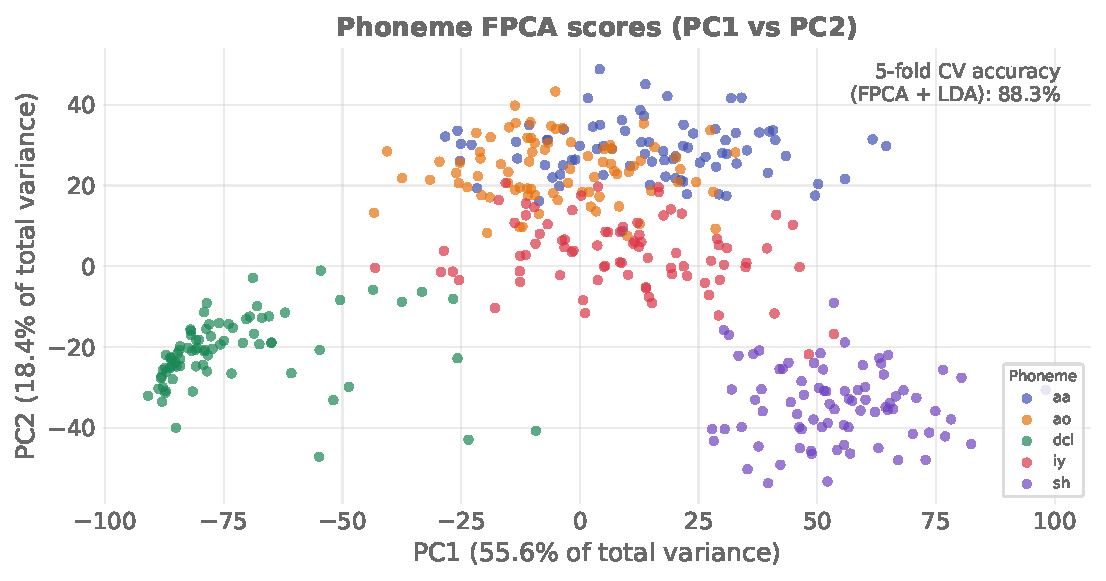
\includegraphics[width=\textwidth]{figures/cs1_phoneme_fpca.pdf}
  \caption{FPCA scores scatter for the phoneme data (PC1 vs PC2, colour-coded
    by class).  The first two principal components explain \csOneVarPCOne\% and
    \csOneVarPCTwo\% of total variance respectively; \textit{dcl},
    \textit{iy} and \textit{sh} are well separated in this projection, while
    \textit{aa} and \textit{ao} overlap.  The box reports the
    \csOneCVAcc\% 5-fold CV accuracy of \texttt{FPCATransformer} +
    \texttt{LinearDiscriminantAnalysis} on \csOneNComp{} components.}
  \label{fig:cs1-fpca}
\end{figure}

% paper/sections/casestudy2.tex — Case Study 2: Tecator (registration, scalar-on-function regression)
% Every number below is a macro written by paper/code/casestudy2.py into
% sections/cs2_numbers.tex (drift gate: paper/code/check_cs_numbers.py).
% Auto-generated by paper/code/casestudy2.py -- do not edit.
% Regenerate: PYTHONPATH=scripts:paper/code python paper/code/casestudy2.py
% Drift gate: PYTHONPATH=scripts:paper/code python paper/code/check_cs_numbers.py
\newcommand{\csTwoNSamples}{240}
\newcommand{\csTwoNChannels}{100}
\newcommand{\csTwoFatMin}{0.9}
\newcommand{\csTwoFatMax}{58.5}
\newcommand{\csTwoNKarcher}{30}
\newcommand{\csTwoKarcherIter}{20}
\newcommand{\csTwoKarcherConverged}{no}
\newcommand{\csTwoNComp}{15}
\newcommand{\csTwoTrainRtwo}{0.974}
\newcommand{\csTwoTrainRtwoRaw}{0.970}
\newcommand{\csTwoCVRtwo}{0.928}
\newcommand{\csTwoCVFolds}{0.934, 0.831, 0.940, 0.971, 0.962}
\newcommand{\csTwoCVRtwoRaw}{0.916}
\newcommand{\csTwoCVRtwoRegRaw}{-0.017}
\newcommand{\csTwoCVRtwoRegDtwo}{0.210}
\newcommand{\csTwoNShown}{30}


\subsection{Registration and Scalar-on-Function Regression: Tecator Data}
\label{subsec:cs2-tecator}

The tecator dataset consists of \csTwoNSamples{} near-infrared absorbance spectra of meat
samples measured at \csTwoNChannels{} spectral channels, with fat content (ranging from
\csTwoFatMin\% to \csTwoFatMax\%) recorded as a scalar response for each sample
\citep{borggaard_thodberg_1992}.  This study pairs two \texttt{fdars}
capabilities---elastic registration under the square-root slope function
(SRSF) framework \citep{srivastava_klassen_2016} and scalar-on-function
functional principal component regression \citep{reiss_ogden_2007}---and uses
the pair to make a methodological point: registration should be applied only
when phase variation is a nuisance, and in near-infrared spectra it is not.

\paragraph{Registration.}
We estimate an elastic Karcher mean from a representative subset of \csTwoNKarcher{} curves
using \texttt{fdars.alignment.karcher\_mean}, with the Fisher--Rao gradient
descent capped at \csTwoKarcherIter{} iterations for speed (it had not met its tolerance when
stopped), and align all \csTwoNSamples{} spectra to that mean with
\texttt{fdars.alignment.align\_to\_target}.  Figure~\ref{fig:cs2-align} shows
the effect: the absorption peak is pulled to a common location across samples.

\paragraph{Scalar-on-function regression.}
Following standard near-infrared practice~\citep{rinnan_2009}, we convert the absorbance curves to
\emph{second-derivative} spectra---B-spline smoothing followed by double
differentiation---which removes additive baseline offsets and linear baseline
slopes (the additive part of light-scatter effects; multiplicative scatter is
not corrected).  Fat content is
then modelled as a linear functional of the second-derivative spectrum via FPC
regression (\texttt{fdars.regression.fregre\_lm}, \csTwoNComp{} components).
Fitting on all \csTwoNSamples{} samples gives a training $R^2 = \csTwoTrainRtwo$
(Figure~\ref{fig:cs2-fit}); the same model on the raw absorbance spectra gives
$R^2 = \csTwoTrainRtwoRaw$.

\paragraph{Cross-validation.}
Five-fold cross-validation of \texttt{FPCRegressor} (\csTwoNComp{} components) via
\texttt{sklearn.\allowbreak model\_selection.\allowbreak cross\_val\_score}
gives a mean $R^2 = \csTwoCVRtwo$ on second-derivative spectra (folds
$[\csTwoCVFolds]$) against $\csTwoCVRtwoRaw$ on the raw spectra---a
small but consistent gain from the preprocessing.

\paragraph{Should the spectra be registered first?}
No.  Repeating the cross-validation on the \emph{registered} spectra drops the
mean $R^2$ to $\csTwoCVRtwoRegRaw$ for the absorbance curves and $\csTwoCVRtwoRegDtwo$ for their second
derivatives.  The positions and shapes of the absorption bands encode the
chemical composition, so the warping that aligns them removes precisely the
information that predicts fat content.  The registration step is therefore
shown as an illustration of the alignment interface, not as preprocessing for
this regression; in applications where timing is a nuisance (such as the
growth-velocity curves in Section~\ref{sec:capabilities}), the same interface
is the right tool.
The complete analysis, including every number above, is reproduced by
\texttt{paper/code/casestudy2.py}.

\begin{figure}[tbp]
  \centering
  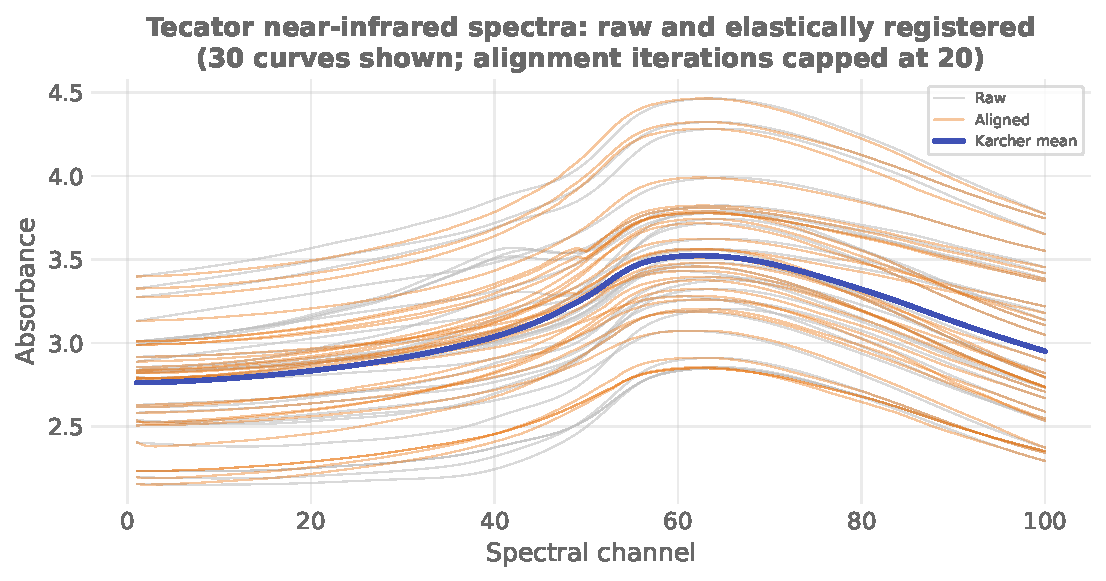
\includegraphics[width=\textwidth]{figures/cs2_tecator_align.pdf}
  \caption{Tecator near-infrared spectra before and after elastic SRSF
    registration (\csTwoNShown{} of \csTwoNSamples{} curves shown).  Grey traces: raw spectra.
    Coloured traces: spectra aligned to the Karcher mean.  Bold trace: the
    estimated Karcher mean used as the registration target (iterations capped
    at \csTwoKarcherIter).  Aligning the absorption peak removes the predictive signal
    (see text).}
  \label{fig:cs2-align}
\end{figure}

\begin{figure}[tbp]
  \centering
  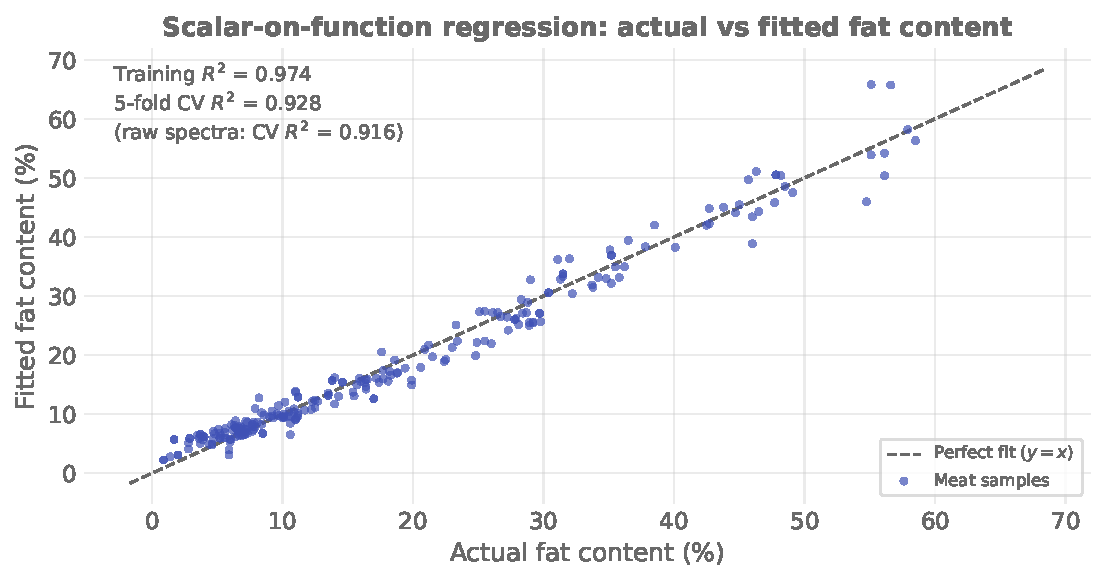
\includegraphics[width=\textwidth]{figures/cs2_tecator_fit.pdf}
  \caption{Scalar-on-function FPC regression on the tecator data: actual
    versus fitted fat content for all \csTwoNSamples{} meat samples, using unregistered
    second-derivative spectra (\texttt{fdars.regression.fregre\_lm},
    \csTwoNComp{} components).  The dashed line marks perfect prediction ($y = x$).
    Training $R^2 = \csTwoTrainRtwo$; 5-fold CV $R^2 = \csTwoCVRtwo$ (raw spectra: $\csTwoCVRtwoRaw$).}
  \label{fig:cs2-fit}
\end{figure}

% paper/sections/casestudy3.tex — Case Study 3: FTS forecasting of PM10 air pollution.
% Revised in the pre-arXiv review pass; all numbers are printed by paper/code/casestudy3.py.

\subsection{Functional Time Series Forecasting: Daily PM10 Air Pollution}
\label{subsec:cs3-fts}

The Graz PM10 dataset~\citep{aue_norinho_hormann_2015} records the
concentration of airborne particulate matter (aerodynamic diameter
$<10\,\mu$m, in $\mu$g/m$^3$) at half-hourly resolution at the Graz-Mitte
station, from 2010-10-01 to 2011-03-31.  Reshaping the record into one curve
per day gives a genuine functional time series: 182 consecutive daily curves,
each a 48-point diurnal PM10 profile.  Unlike a cross-sectional collection, the
curves are ordered in real calendar time, so forecasting \emph{the next day's}
pollution profile is a substantive task~\citep{hyndman_ullah_2007,hormann_kokoszka_2010}.
Following \citet{aue_norinho_hormann_2015}, we model the data on the
variance-stabilising square-root scale and back-transform forecasts to
$\mu$g/m$^3$.

\paragraph{Model.}
\texttt{fdars.fts.ftsm(X, ARG, ncomp=3)} fits the functional principal
component decomposition of the curve sequence and an independent univariate
autoregressive model to each of the three score series (Yule--Walker
estimation, order chosen by AIC); \texttt{fdars.\allowbreak fts.\allowbreak
ftsm\_forecast} forecasts the scores and reconstructs the curves.
Figure~\ref{fig:cs3-curves} shows the 182 daily curves together with the FTS
mean, exposing the diurnal structure and the wide day-to-day amplitude
variation the model must capture.

\paragraph{Rolling-origin validation.}
A single train/test split is a fragile basis for judging a forecaster, so we
use a rolling origin.  For each of the last 30 possible forecast origins
(first forecast days 2011-02-24 to 2011-03-25) we fit the model on all days
before the origin and forecast seven days ahead.  Each forecast curve is
compared to the actual curve by root-mean-square error (RMSE, $\mu$g/m$^3$),
against two baselines: \emph{climatology} (the mean curve of the days before
the origin) and \emph{persistence} (the day before the origin).
At the one-day-ahead horizon the FTS forecast attains a mean RMSE of $17.69$,
against $26.18$ for climatology and $20.82$ for persistence; it beats
climatology at 26 and persistence at 20 of the 30 origins.  Averaged over all
seven horizons the mean RMSE is $21.32$ (FTS), $24.23$ (climatology), and
$27.02$ (persistence).  Figure~\ref{fig:cs3-forecast} shows the one-day-ahead
forecast at the final origin (left) and the mean RMSE at each horizon with
$\pm1$ standard-error bands (right).  The full analysis is reproduced by
\texttt{paper/code/casestudy3.py}.

\paragraph{Honest caveat.}
Forecast skill decays with horizon: the advantage over climatology is clear at
one day ahead but narrows to about one $\mu$g/m$^3$ at seven days, where a
low-rank curve model cannot anticipate day-specific pollution events.  The
study demonstrates that \texttt{fdars}' FTS interface produces skilful
next-day functional forecasts on a real temporal dataset; it is not a claim of
state-of-the-art air-quality forecasting.

\begin{figure}[tbp]
  \centering
  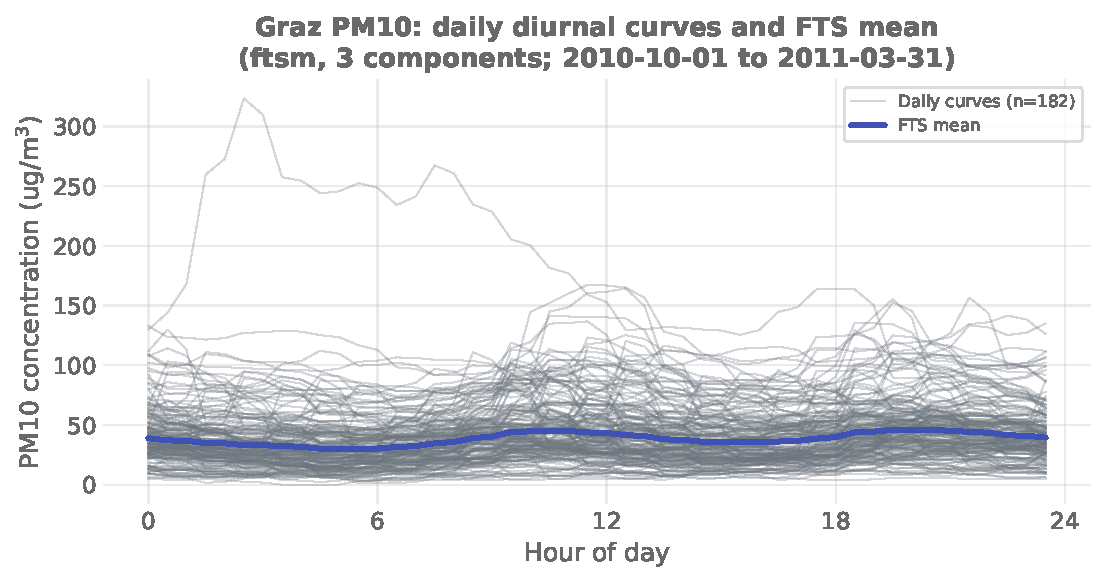
\includegraphics[width=\textwidth]{figures/cs3_pm10_curves.pdf}
  \caption{Graz PM10: the 182 daily diurnal curves (grey) and the FTS mean
    curve (solid, \texttt{ftsm}, 3 components).  Each day contributes one
    48-point functional observation; the $x$-axis is the hour of day.}
  \label{fig:cs3-curves}
\end{figure}

\begin{figure}[tbp]
  \centering
  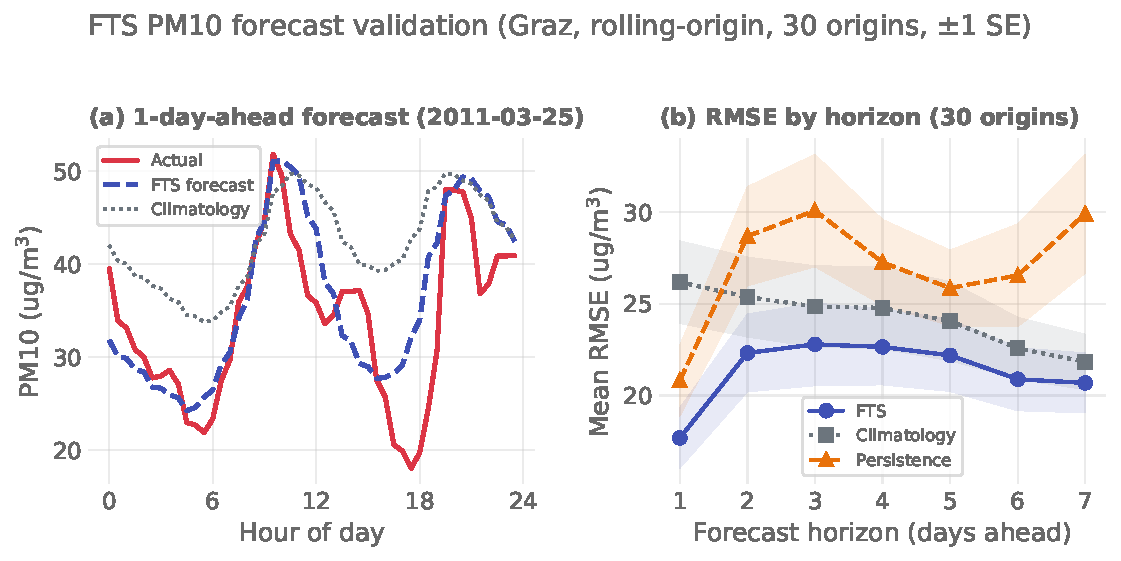
\includegraphics[width=\textwidth]{figures/cs3_pm10_forecast.pdf}
  \caption{Rolling-origin validation of the FTS PM10 forecast (30 origins).
    \emph{Left:} the one-day-ahead forecast at the final origin (2011-03-25)
    against the actual curve and the climatology baseline.  \emph{Right:} mean
    RMSE ($\mu$g/m$^3$) at each horizon for the FTS model, climatology, and
    persistence, with $\pm1$ standard-error bands.}
  \label{fig:cs3-forecast}
\end{figure}

% paper/sections/casestudy4.tex — Case Study 4: Berkeley growth (composable sklearn Pipeline + nested GridSearchCV)
% Every number below is a macro written by paper/code/casestudy4.py into
% sections/cs4_numbers.tex (drift gate: paper/code/check_cs_numbers.py).
% Auto-generated by paper/code/casestudy4.py -- do not edit.
% Regenerate: PYTHONPATH=scripts:paper/code python paper/code/casestudy4.py
% Drift gate: PYTHONPATH=scripts:paper/code python paper/code/check_cs_numbers.py
\newcommand{\csFourNChildren}{93}
\newcommand{\csFourNBoys}{39}
\newcommand{\csFourNGirls}{54}
\newcommand{\csFourNAges}{31}
\newcommand{\csFourAgeMin}{1}
\newcommand{\csFourAgeMax}{18}
\newcommand{\csFourGrid}{2, 3, 4, 6}
\newcommand{\csFourNInner}{5}
\newcommand{\csFourNOuter}{5}
\newcommand{\csFourNRep}{10}
\newcommand{\csFourNOuterFolds}{50}
\newcommand{\csFourHeightTwo}{0.967}
\newcommand{\csFourHeightThree}{0.957}
\newcommand{\csFourHeightFour}{0.957}
\newcommand{\csFourHeightSix}{0.967}
\newcommand{\csFourVelocityTwo}{0.894}
\newcommand{\csFourVelocityThree}{0.882}
\newcommand{\csFourVelocityFour}{0.925}
\newcommand{\csFourVelocitySix}{0.957}
\newcommand{\csFourBestRep}{height}
\newcommand{\csFourBestK}{2}
\newcommand{\csFourBestKWord}{two}
\newcommand{\csFourNested}{0.970}
\newcommand{\csFourNestedSd}{0.036}
\newcommand{\csFourBaseEighteen}{0.862}
\newcommand{\csFourBaseEighteenSd}{0.058}
\newcommand{\csFourBaseTwo}{0.962}
\newcommand{\csFourBaseTwoSd}{0.043}
\newcommand{\csFourAgeEarly}{12}


\subsection{Composable scikit-learn Pipelines: Berkeley Growth Data}
\label{subsec:cs4-growth}

This study showcases the \emph{composability} of the \texttt{fdars}
scikit-learn layer on a genuinely functional problem: predicting a child's sex
from their growth curve.  The Berkeley growth study
\citep{tuddenham_snyder_1954}, in the version distributed with the R
\texttt{fda} package \citep{r_fda} and analysed by
\citet{ramsay_silverman_2005}, records the heights of
\csFourNChildren{} children (\csFourNBoys{} boys, \csFourNGirls{} girls) at
\csFourNAges{} ages between \csFourAgeMin{} and \csFourAgeMax{} years.  Adult height alone separates the
sexes only partly; the timing of the pubertal growth spurt---earlier in
girls---carries additional information that a curve-level method can use.

\paragraph{Pipeline and search.}
The pipeline chains three steps: an optional representation step (either the
height curves themselves or growth-velocity curves, obtained by GCV B-spline
smoothing and differentiation with \texttt{fdars} functions wrapped in a
scikit-learn \texttt{FunctionTransformer}), an \texttt{fdars}
\texttt{FPCATransformer}, and scikit-learn's own
\texttt{LinearDiscriminantAnalysis}.  \texttt{GridSearchCV} treats the
representation as an ordinary hyperparameter alongside the number of FPCA
components, $\{\csFourGrid\}$, using seeded stratified \csFourNInner-fold
cross-validation.  No adapter code is needed: every step obeys the
scikit-learn estimator contract.

\paragraph{Results.}
Height curves score higher than velocity curves at every dimension
(Figure~\ref{fig:cs4-gridsearch}; mean inner CV accuracy $\csFourHeightTwo$, $\csFourHeightThree$,
$\csFourHeightFour$, $\csFourHeightSix$ for $\csFourGrid$ components, against
$\csFourVelocityTwo$, $\csFourVelocityThree$, $\csFourVelocityFour$,
$\csFourVelocitySix$ for velocity), and the search selects \csFourBestRep{}
curves with \csFourBestKWord{} components\csFourBestTie{}.  Because a score used for selection is optimistically biased, we
evaluate the \emph{entire} search by nested cross-validation (an outer
stratified \csFourNOuter-fold split repeated \csFourNRep{} times).  Because the
inner search may choose different configurations in different outer folds,
this scores the complete selection procedure rather than one fixed pipeline:
it attains a mean accuracy of $\csFourNested$ (standard deviation
$\csFourNestedSd$ across the \csFourNOuterFolds{} outer folds).  Under the
identical outer splits, a logistic regression on final height alone reaches
$\csFourBaseEighteen$ (s.d.\ $\csFourBaseEighteenSd$), and one on the heights at
ages \csFourAgeEarly{} and \csFourAgeMax---an expert's hand-picked
``before and after puberty'' pair---reaches $\csFourBaseTwo$
(s.d.\ $\csFourBaseTwoSd$).  The functional
pipeline thus matches the expert feature choice without being told which ages
matter.  Figure~\ref{fig:cs4-scores} shows why \csFourBestKWord{} components suffice: the
first is an overall size mode and the second a growth-timing mode (compare
Figure~\ref{fig:tour-fpca}), and together they separate boys from girls
almost linearly.
The analysis is reproduced by \texttt{paper/code/casestudy4.py}.

\begin{figure}[tbp]
  \centering
  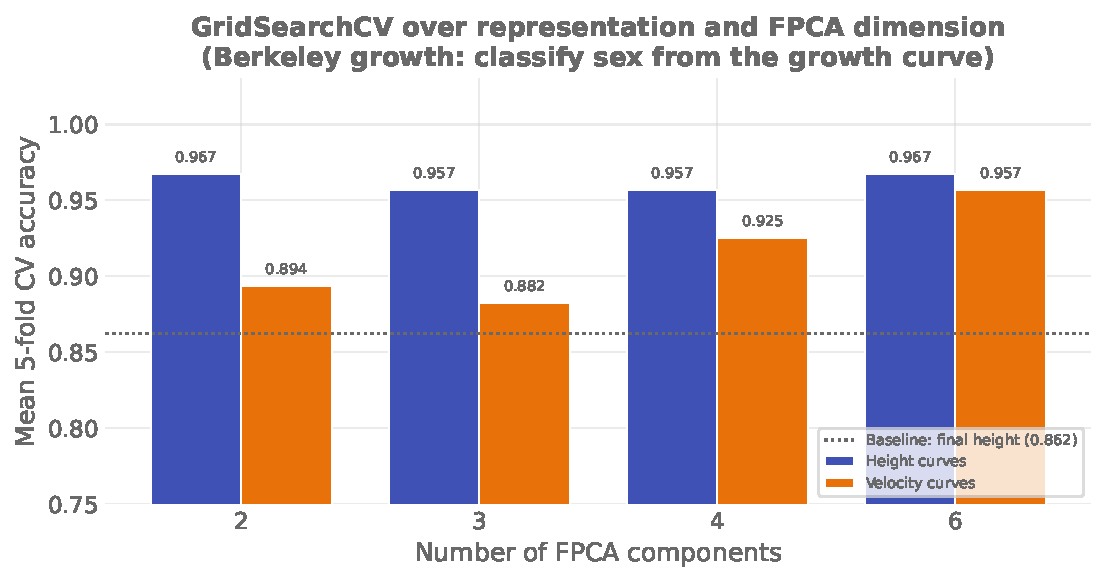
\includegraphics[width=\textwidth]{figures/cs4_growth_gridsearch.pdf}
  \caption{\texttt{GridSearchCV} over the functional representation (height
    or velocity curves) and the number of FPCA components, for the pipeline
    representation $\to$ \texttt{FPCATransformer} $\to$
    \texttt{LinearDiscriminantAnalysis}.  Bars show the mean inner
    \csFourNInner-fold CV accuracy of the grid search (one seeded split of the
    full sample); the dotted line is a logistic regression on final height
    alone, scored by the repeated (\csFourNRep$\times$\csFourNOuter-fold) outer
    CV, so the two are not scored on identical splits.}
  \label{fig:cs4-gridsearch}
\end{figure}

\begin{figure}[tbp]
  \centering
  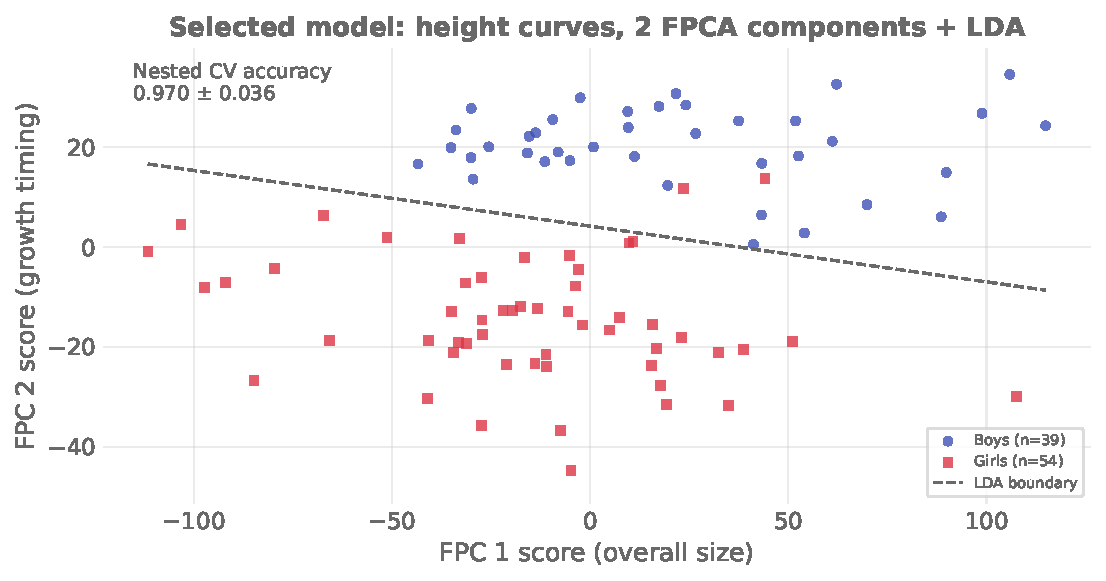
\includegraphics[width=\textwidth]{figures/cs4_growth_scores.pdf}
  \caption{FPCA scores of the selected model (\csFourBestRep{} curves,
    \csFourBestKWord{} components),
    coloured by sex, with the LDA decision boundary.  The first component
    reflects overall size and the second the timing of the growth spurt; the
    box reports the nested cross-validated accuracy of the whole search (mean
    $\pm$ standard deviation over the \csFourNOuterFolds{} outer folds).}
  \label{fig:cs4-scores}
\end{figure}

